% ------------------------------------------------------------------------------
% TYPO3 CMS 8.5 - What's New - Chapter "In-Depth Changes" (French Version)
%
% @author	Michael Schams <schams.net>
% @license	Creative Commons BY-NC-SA 3.0
% @link		http://typo3.org/download/release-notes/whats-new/
% @language	French
% ------------------------------------------------------------------------------
% LTXE-CHAPTER-UID:		5ebcecbe-66abfa57-cf38bc00-aa637965
% LTXE-CHAPTER-NAME:	Changements en profondeur
% ------------------------------------------------------------------------------

\section{Changements en profondeur}
\begin{frame}[fragile]
	\frametitle{Changements en profondeur}

	\begin{center}\huge{Chapitre 3~:}\end{center}
	\begin{center}\huge{\color{typo3darkgrey}\textbf{Changements en profondeur}}\end{center}

\end{frame}

% ------------------------------------------------------------------------------
% LTXE-SLIDE-START
% LTXE-SLIDE-UID:		bde270e6-ffef8544-ea472ed5-89ba8c3d
% LTXE-SLIDE-TITLE:		#78581: FormEngine Data Providers
% ------------------------------------------------------------------------------

\begin{frame}[fragile]
	\frametitle{Changements en profondeur}
	\framesubtitle{Fournisseur de données FormEngine}

	\begin{itemize}
		\item Le fournisseur de données FormEngine \texttt{TcaFlexFetch} est
			fusionné dans \texttt{TcaFlexPrepare}
		\item Cela affecte seulement les instances dans le cas rare où un fournisseur
			de donnée personnalisé déclare une dépendance envers \texttt{TcaFlexFetch}
	\end{itemize}

\end{frame}

% ------------------------------------------------------------------------------
% LTXE-SLIDE-START
% LTXE-SLIDE-UID:		f0fb603c-54e9f255-03140395-b6b18103
% LTXE-SLIDE-TITLE:		#78384: Frontend ignores TCA in ext_tables.php
% ------------------------------------------------------------------------------
\begin{frame}[fragile]
	\frametitle{Changements en profondeur}
	\framesubtitle{TCA dans \texttt{ext\_tables.php}}

	\begin{itemize}
		\item Les requêtes frontend ne chargent plus les \texttt{ext\_tables.php}
		\item Impacte les extensions configurant du TCA dans \texttt{ext\_tables.php}\newline
			\small(qui n'était déjà plus autorisé)\normalsize
		\item L'outil d'installation fourni un test "Vérification TCA ext\_tables" pour
			identifier ces extensions
	\end{itemize}

	\begin{figure}
		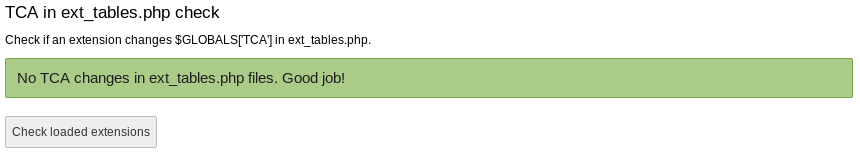
\includegraphics[width=0.95\linewidth]{InDepthChanges/78384-install-tool-tca-in-exttables-check.png}
	\end{figure}

\end{frame}
% ------------------------------------------------------------------------------
% LTXE-SLIDE-START
% LTXE-SLIDE-UID:		bdcd2449-b679717b-9f23eb32-018953b4
% LTXE-SLIDE-TITLE:		#78191: Remove support for transForeignTable/transOrigPointerTable in TCA
% ------------------------------------------------------------------------------
\begin{frame}[fragile]
	\frametitle{Changements en profondeur}
	\framesubtitle{TCA dans \texttt{ext\_tables.php}}

	\begin{itemize}
		\item Les tables des bases qui contenaient les enregistrements de localisation
			et traduction étaient configurable en TCA

			\begin{itemize}
				\item \texttt{\$TCA[<table\_name>]['ctrl']['transForeignTable']}\newline
					(ciblait habituellement~: \texttt{pages\_language\_overlay})
				\item \texttt{\$TCA[<table\_name>]['ctrl']['transOrigPointerTable']}\newline
					(ciblait habituellement~: \texttt{pages})
			\end{itemize}

		\item Cette configuration est remplacée par le nom des tables en dur pour
			empêcher le traitement particulier et préparer pour la fusion future
			de ces tables

	\end{itemize}

\end{frame}

% ------------------------------------------------------------------------------
% LTXE-SLIDE-START
% LTXE-SLIDE-UID:		ede02440-cafd3417-eb416f09-8e024ef2
% LTXE-SLIDE-TITLE:		#78383: Tables removed from defaultCategorizedTables
% ------------------------------------------------------------------------------
\begin{frame}[fragile]
	\frametitle{Changements en profondeur}
	\framesubtitle{Tables retirées de \texttt{defaultCategorizedTables}}

	\begin{itemize}
		\item Les tables suivantes ont été retirées de \texttt{defaultCategorizedTables}~:

			\begin{itemize}
				\item \texttt{pages}
				\item \texttt{tt\_content}
				\item \texttt{sys\_file\_metadata}
			\end{itemize}

		\item Pour ces tables, la méthode du noyau\newline
			\texttt{ExtensionManagementUtility::makeCategorizable()}\newline
			est exécutée pour définir une position commune du champ de
			catégories

	\end{itemize}

\end{frame}


% ------------------------------------------------------------------------------
% LTXE-SLIDE-START
% LTXE-SLIDE-UID:		dd31e5d5-ca09ae5e-eb87d926-0ffe8f0a
% LTXE-SLIDE-TITLE:		Low-level parameters changes (1)
% ------------------------------------------------------------------------------
\begin{frame}[fragile]
	\frametitle{Changements en profondeur}
	\framesubtitle{Changement de paramètres low-level (1)}

	% changes: #78417, #78439, #78520, #78552, #78577, #78623, #78627 and #78895

	\begin{itemize}
		\item Les commandes low-level ci-dessous utilisent la console Symfony
		\item Les nouvelles commandes se comportent comme les anciennes mais
			leurs paramètres sont spécifiés différemment

			\begin{itemize}
				\item \texttt{DeletedRecordsCommand}
				\item \texttt{CleanFlexFormsRecordsCommand}
				\item \texttt{OrphanRecordsCommand}
				\item \texttt{LostFilesCommand}
				\item \texttt{MissingFilesCommand}
				\item \texttt{MissingRelationsCommand}
				\item \texttt{DoubleFilesCommand}
				\item \texttt{RteImagesCommand}
			\end{itemize}

	\end{itemize}

\end{frame}



% ------------------------------------------------------------------------------
% LTXE-SLIDE-START
% LTXE-SLIDE-UID:		3a9d25bb-d948368d-e2a92666-6170eaad
% LTXE-SLIDE-TITLE:		Low-level parameters changes (2)
% ------------------------------------------------------------------------------
\begin{frame}[fragile]
	\frametitle{Changements en profondeur}
	\framesubtitle{Changement de paramètres low-level (2)}

	% changes: #78417, #78439, #78520, #78552, #78577, #78623, #78627 and #78895

	\begin{itemize}
		\item Les classes associées sont retirées\newline
			\smaller(ex. \texttt{TYPO3\textbackslash
				CMS\textbackslash
				Lowlevel\textbackslash
				DeletedRecordsCommand})
			\normalsize

		\item Exécuter la commande via \texttt{cli\_dispatch} ne fonctionne plus\newline
			\smaller(ex. \texttt{typo3/cli\_dispatch lowlevel cleaner deleted})\normalsize
		\item Appeler ces classes PHP résulte en une erreur fatale

		\item Les commandes s'exécutent via CLI comme suit~:\newline
			\smaller\texttt{/typo3/sysext/core/bin/typo3 cleanup:<command>}\normalsize\newline
			par exemple~:\newline
			\smaller\texttt{/typo3/sysext/core/bin/typo3 cleanup:deletedrecords}\normalsize

	\end{itemize}

\end{frame}




% ------------------------------------------------------------------------------
% LTXE-SLIDE-START
% LTXE-SLIDE-UID:		ec6817fd-c3364ffb-c74e9523-a18a3095
% LTXE-SLIDE-TITLE:		Re-factor FlexForm Data Structure Handling
% ------------------------------------------------------------------------------
\begin{frame}[fragile]
	\frametitle{Changements en profondeur}
	\framesubtitle{Refactorisation du traitement des structures de données FlexForm}

	% https://forge.typo3.org/issues/78581
	% https://forge.typo3.org/issues/78616
	% https://forge.typo3.org/issues/78852
	% https://forge.typo3.org/issues/69715

	\begin{itemize}
		\item Avec la dépréciation de \texttt{BackendUtility::getFlexFormDS()}, le hook
			\texttt{getFlexFormDSClass} n'est plus appelé

	\end{itemize}

\end{frame}





% ------------------------------------------------------------------------------
% LTXE-SLIDE-START
% LTXE-SLIDE-UID:		b400c3b8-3e402480-cd7d6ff3-96cd93aa
% LTXE-SLIDE-TITLE:		#76085: Add fluid debug information to admin panel
% ------------------------------------------------------------------------------
\begin{frame}[fragile]
	\frametitle{Changements en profondeur}
	\framesubtitle{Panneau d'administration}

	\begin{itemize}
		\item La panneau d'administration contient une nouvelle option de déboggage
			de la sortie Fluid~:
			\textbf{Prévisualisation -> Afficher la sortie de déboggage fluid}
		\item Si activé, les détails suivant sont affichés en frontend~:

			\begin{itemize}
				\item chemin vers le fichier d'un partial
				\item nom de la section
			\end{itemize}

		\item Cette fonction permet aux intégrateurs de repérer facilement les bons template
			section

	\end{itemize}

\end{frame}






% ------------------------------------------------------------------------------
% LTXE-SLIDE-START
% LTXE-SLIDE-UID:		60a2d39f-f04b8bf1-dc758912-607ed07e
% LTXE-SLIDE-TITLE:		#52286: System Status Updates Report via email
% ------------------------------------------------------------------------------
\begin{frame}[fragile]
	\frametitle{Changements en profondeur}
	\framesubtitle{État de mise à jour système (Rapports)}

	\begin{itemize}
		\item Les résultats du test «~État de mise à jour système (Rapports)~» peuvent
			être envoyés par email
		\item Une case à cocher est ajoutée à la configuration pour~:

			\begin{itemize}
				\item envoyer un email s'il y a des erreurs ou avertissements
				\item toujours envoyer un email
			\end{itemize}

		\item La valeur par défaut est de n'inclure que les erreurs et avertissements

	\end{itemize}

\end{frame}







% ------------------------------------------------------------------------------
% LTXE-SLIDE-START
% LTXE-SLIDE-UID:		e4e2ead3-c07beb21-e8100580-d0e7c756
% LTXE-SLIDE-TITLE:		#58637: Purge language packs in language module
% ------------------------------------------------------------------------------
\begin{frame}[fragile]
	\frametitle{Changements en profondeur}
	\framesubtitle{Packs de langue}

	\begin{itemize}
		\item Désactiver une langue dans le module "Langues" laissait les données
			de la langue dans le dossier \texttt{typo3conf/l10n/<locale>/}
		\item Un bouton "supprimer" est ajouté, désactivant la langue et purgeant
			les données du dossier
	\end{itemize}

\end{frame}








% ------------------------------------------------------------------------------
% LTXE-SLIDE-START
% LTXE-SLIDE-UID:		08961fb3-00cbc9f4-964f8d01-6e59e782
% LTXE-SLIDE-TITLE:		#67909: Hook added to localize() function
% ------------------------------------------------------------------------------
\begin{frame}[fragile]
	\frametitle{Changements en profondeur}
	\framesubtitle{Hook dans DataHandler \texttt{localize()}}

	% decrease font size for code listing
	\lstset{basicstyle=\tiny\ttfamily}

	\begin{itemize}
		\item Un hook est ajouté à la fonction \texttt{localize()}
		\item Permet d'utiliser par exemple un service de traduction externe ou des
			fonctions de transliteration personnalisée qui gérent diverses transformations
			du contenu
	\end{itemize}

	\begin{itemize}
		\item Hook~:\newline
			\smaller
				\texttt{\$GLOBALS['TYPO3\_CONF\_VARS']['SC\_OPTIONS']\newline
				\tabto{0.4cm}['t3lib/class.t3lib\_tcemain.php']['processTranslateToClass']}
			\normalsize

		\item Exemple d'usage~:

			\begin{lstlisting}
				class YourHookClass
				{
				  public function processTranslateTo_copyAction(&$content, $lang, $dataHandler)
				  {
				    // Do something with content (translate, transliterate etc.)
				  }
				}
			\end{lstlisting}
	\end{itemize}

\end{frame}









% ------------------------------------------------------------------------------
% LTXE-SLIDE-START
% LTXE-SLIDE-UID:		8b1a9661-d6fab90f-9c856224-ee663aa2
% LTXE-SLIDE-TITLE:		#77757: Re-check if an UpdateWizard should run
% ------------------------------------------------------------------------------
\begin{frame}[fragile]
	\frametitle{Changements en profondeur}
	\framesubtitle{Assistant de mise à jour}

	\begin{columns}[T]
		\begin{column}{.5\textwidth}
			L'assistant de mise à jour de l'outil d'installation liste
			toutes les tâches marquées \textit{réalisée}.
			\newline\newline
			Des cases et un bouton "Revérifier les assistants choisis"
			permet de réinitier les mises à jour.
			L'assistant vérifiera si la tâche a besoin d'être exécutée de nouveau.
		\end{column}
		\begin{column}{.5\textwidth}
			\begin{figure}\vspace*{-0.5cm}
				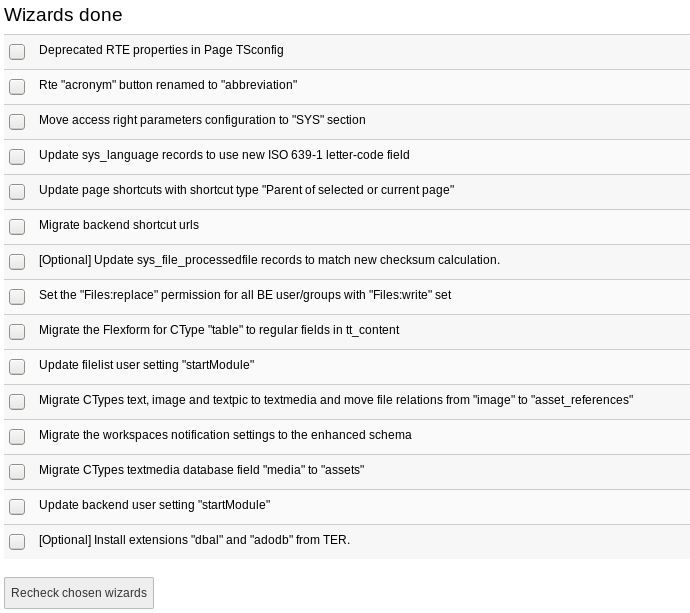
\includegraphics[width=0.8\linewidth]{InDepthChanges/77757-upgrade-wizard.png}
			\end{figure}
		\end{column}
	\end{columns}

\end{frame}









% ------------------------------------------------------------------------------
% LTXE-SLIDE-START
% LTXE-SLIDE-UID:		94640f3d-0f632507-a2166719-5adc755e
% LTXE-SLIDE-TITLE:		#78523: Suggest wizard provides option to define ordering of results
% ------------------------------------------------------------------------------
\begin{frame}[fragile]
	\frametitle{Changements en profondeur}
	\framesubtitle{Assistant suggestion}

	% decrease font size for code listing
	\lstset{basicstyle=\tiny\ttfamily}

	\begin{itemize}
		\item Le FormEngine ("TCEforms") permet de configurer l'ordre des
			résultats de l'assistant suggestion
		\item La nouvelle option est une définition standard de clause SQL order-by~:\newline
			\small\texttt{'orderBy' => 'field ASC/DESC'}\normalsize
		\item Exemple de configuration TCA~:

			\begin{lstlisting}
				'config' => [
				  ...
				  'wizards' => [
				    'suggest' => [
				      'type' => 'suggest',
				      'default' => [
				        'searchWholePhrase' => true,
				        'addWhere' => ' AND tx_news_domain_model_news.uid != ###THIS_UID###',
				        'orderBy => 'datetime DESC',
				      ]
				    ],
				  ],
				]
			\end{lstlisting}

	\end{itemize}

\end{frame}











% ------------------------------------------------------------------------------
% LTXE-SLIDE-START
% LTXE-SLIDE-UID:		0907e5d3-a12751cb-23f49488-7a05a208
% LTXE-SLIDE-TITLE:		Miscellaneous
% ------------------------------------------------------------------------------
\begin{frame}[fragile]
	\frametitle{Changements en profondeur}
	\framesubtitle{Divers}

	% #78103: Add missing information status for addSystemMessage
	% #78575: Get enumeration constants
	% #75232: Spread TypeConverter priorities

	\begin{itemize}
		\item Toutes les informations systèmes ajoutées par \texttt{addSystemInformation()}
		 	ont la valeur \texttt{InformationStatus::STATUS\_NOTICE} par défaut
		\item Les constantes des énumerations se récupèrent facilement~:

			\begin{itemize}
				\item \texttt{EnumerationClass::getName(\$value);}
				\item \texttt{EnumerationClass::getHumanReadableName(\$value);}
			\end{itemize}

		\item Les priorités des TypeConverter du noyau ont changées de\newline
			\texttt{1}, \texttt{2}, \texttt{3},… à \texttt{10}, \texttt{20}, \texttt{30},…
			Lors de l'inscription de convertisseurs personalisés, veillez à utiliser les
			bonnes priorités

		\item \href{https://en.wikipedia.org/wiki/ISO_8601}{ISO-8601} est utilisé pour passer les
			valeurs de date et date avec heure entre le serveur et le client. Vérifiez si vos types
			personnalisés de FormEngine ont besoin d'être mis à jour (\texttt{eval=date/datetime}).

	\end{itemize}

\end{frame}












% ------------------------------------------------------------------------------
